\chapter{Virtualization Technologies}
The accelerated adoption of Linux in the cloud computing ecosystem spur the demand for dynamic, efficient and flexible ways to virtualize next generation workloads. As in any case, there is no single best solution to this problem. The linux community currently has multiple mature virtualization platforms and leaves the choice to the end-users. This chapter provides a technical insight into the principles behind the operation of three representative solutions, Kernel-based Virtual Machine(KVM), Xen, and Linux Containers.

%General introduction about virtualization. What types of virtualization we are going to talk in this thesis. Introduce LXC, KVM, Xen.
%Write about the technical background behind all three.
%specifically, LXC is an userspace wrapper over the linux containers facility merged into the Linux kernel.
%The idea of KVM and its isolation benefits as it allows running individual kernels for the VMs.
%The fundamental idea of para virtualization on which Xen is based on.

\section{Kernel based Virtual Machines (KVM)}

KVM is representative of a category of virtualization solution known as \emph{full-virtualization}. A full-virtualization solution as shown in Figure \ref{img_full_virt},is one where a set of virtual devices are emulated over a set of physical devices with a \emph{hypervisor} to arbitrate their access by the \emph{virtual machines} aka \emph{guests}.


%Block diagram of a full-virtualization system%\includegraphics[width=110mm]{../../Pictures/full-virt.png} 
\begin{figure}[htbp]
\centering
\includegraphics[width=120mm]{full-virt.png}
\caption{Block Diagram of a full-virtualization system}
\label{img_full_virt}
\end{figure}
A hypervisor is a very critical part of a stable operating environment as it is responsible for managing the memory available to the guests, scheduling the processes, managing the network connections to and from the guests, manage the Input/Output facilities and maintaining security. The KVM solution, being a relatively new entrant into the virtualization scene, chose to build upon the already developed utilities and features by leveraging the mature, time-proven linux kernel to perform the role of the hypervisor. 

Since the majority of the work was offloaded to the linux kernel, and the fact that it exposed a robust, standard and secure interface to run isolated virtual machines, the functionality was merged into the mainstream linux kernel since 2.6.20 (released February 2007) \cite{kvm_linux_kernel}.

KVM in itself is only a part of the complete virtualization solution. It turns the linux kernel into a Virtual Machine Monitor(VMM) or hypervisor which enables several virtual machines to operate simultaneously as if they are running on their own hardware. The emulated virtual devices and the virtual machine itself are created by an independent tool known as QEMU \cite{qemu}. Hence the solution is commonly referred as QEMU-KVM. KVM is packaged as a lightweight kernel module which implements the virtual machines as regular Linux processes and therefore leverages the linux kernel on the host for all the scheduling and device management activities. 




Figure \ref{img_kvm_arch} shows architecture of a server virtualized using QEMU-KVM.

\newpage 
\begin{figure}[htbp]
\centering
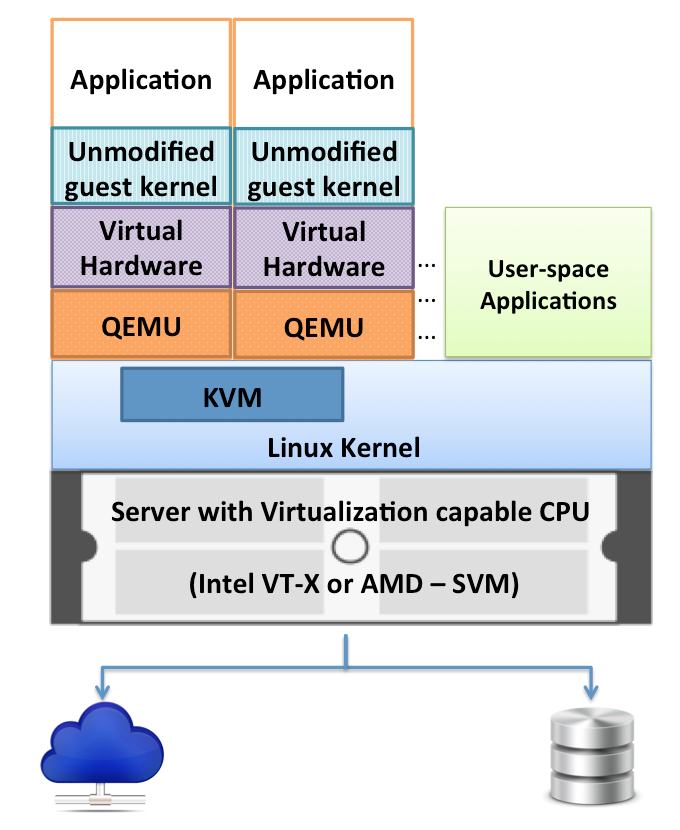
\includegraphics[width=130mm]{kvm-arch.png}
\caption{KVM - Architecture}
\label{img_kvm_arch}
\end{figure}

In practice, KVM and the linux kernel treats a virtual machines a regular Linux process on the host and performs the mapping of virtual devices to the real devices in the following categories.

\begin{enumerate}
\item \textbf{CPU}:

KVM, by design aims at utilizing all possible assistance from the underlying hardware. 
%\begin{wrapfigure}{r}{0.5\textwidth}[htbp]
  %\begin{center}
\begin{figure}[htbp]
\centering
    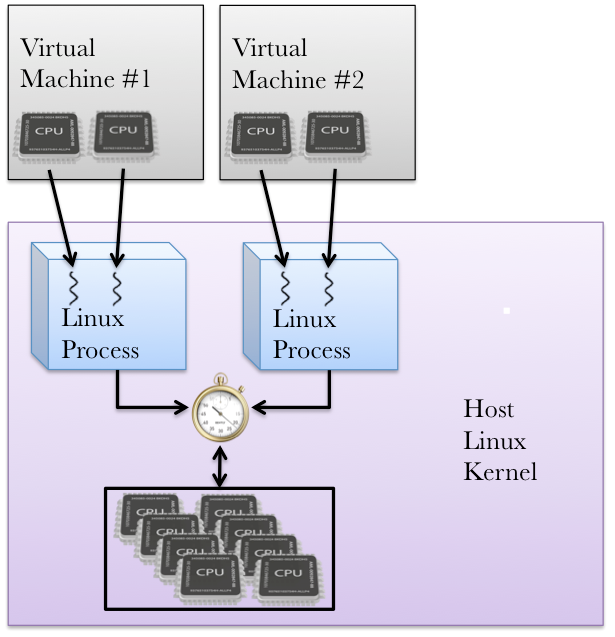
\includegraphics[width=0.48\textwidth]{kvm-cpu.png}
  %\end{center}
  \caption{KVM - Virtual CPU management}
\end{figure}
%\end{wrapfigure}
It requires the CPU to be virtualization aware. Intel VT-X \cite{intelvtx} and AMD-SVM \cite{amdv} are the virtualization extensions provided by Intel and AMD which are the most common variety of CPUs used in the x86 servers, and KVM relies on these facilities to isolate the instructions from the guest operating systems from those from the host itself. Every virtual CPU associated with a virtual machine is created as a thread belonging to the virtual machine's process on the host. Hence, enabling multiple virtual CPUs improve the virtual machine's performance by utilizing the multi-threading facilities on the host. The virtual machine's CPU requests are scheduled by the host kernel using the regular CPU scheduling policies. Improving the CPU performance on the guest and ensuring fair CPU entitlement for the guests are discussed in the later sections.   

\item \textbf{Memory}:

KVM inherits the memory management facilities in the Linux kernel. The memory of a virtual machine is an abstraction of the virtual memory of the standard Linux process on the host. This memory can be swapped, shared with other processes, merged, intelligently managed by the Linux kernel. Thus total of the memory associated with all the virtual machines on a host can be greater than the physical memory available on the host. This feature is known as memory over-committing. Though memory over-commitment increases overall memory utilization, it turns to be a performance problem when all the virtual machines try to utilize their memory share at the same time leading swapping on the host. Since KVM offloads the memory management to the linux kernel, it enjoys the support for NUMA (Non Uniform Memory Access) awareness \cite{numa} and Huge pages \cite{huge_pages} to optimize the memory allocated to the virtual machines. NUMA support and Huge pages will be discussed in the later sections.
   
\item \textbf{Network interfaces}:

Networking in a virtualized infrastructure enables an additional layer of convenience and control over the conventional networking practices. Virtual machines can be networked to the host, co-located virtual machines, or even participate in the same network segment as the host. Several configurations are possible based on the trade-off between compatibility and performance. 



\begin{figure}
        \centering
        \begin{subfigure}[b]{0.35\textwidth}
                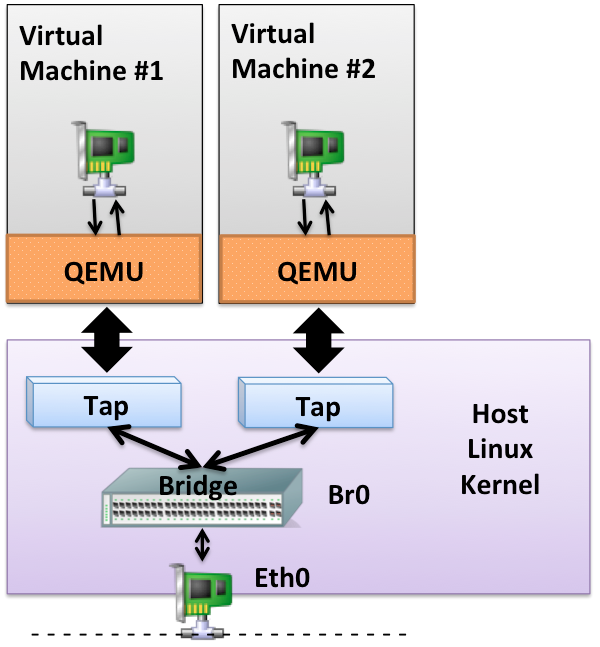
\includegraphics[width=\textwidth]{kvm-emulated.png}
                \caption{KVM - Emulated Networking devices}
                \label{fig:kvm-emulated}
        \end{subfigure}%
        ~ %add desired spacing between images, e. g. ~, \quad, \qquad etc.
        \qquad \hspace{8 mm}
          %(or a blank line to force the subfigure onto a new line)
        \begin{subfigure}[b]{0.35\textwidth}
                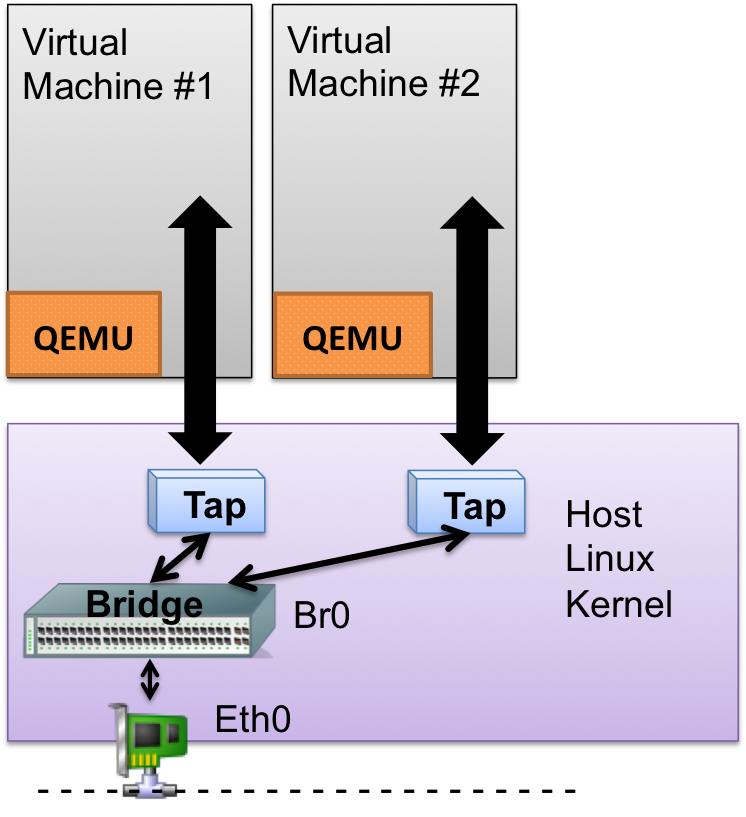
\includegraphics[width=\textwidth]{kvm-para.png}
                \caption{KVM - Para-Virtualized Networking}
                \label{fig:kvm-para}
        \end{subfigure}
        ~ %add desired spacing between images, e. g. ~, \quad, \qquad etc.
\newline \newline
          %(or a blank line to force the subfigure onto a new line)
        \begin{subfigure}[b]{0.35\textwidth}
                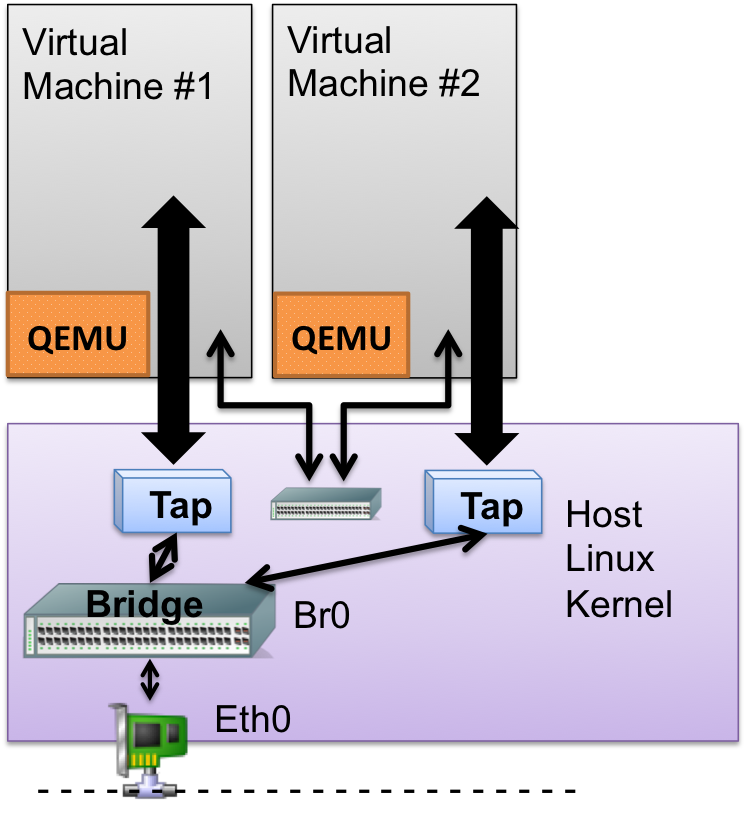
\includegraphics[width=\textwidth]{kvm-internal.png}
                \caption{Public and Private Networking}
                \label{fig:kvm-internal}
        \end{subfigure}
        \quad \hspace{8 mm}
        \begin{subfigure}[b]{0.35\textwidth}
                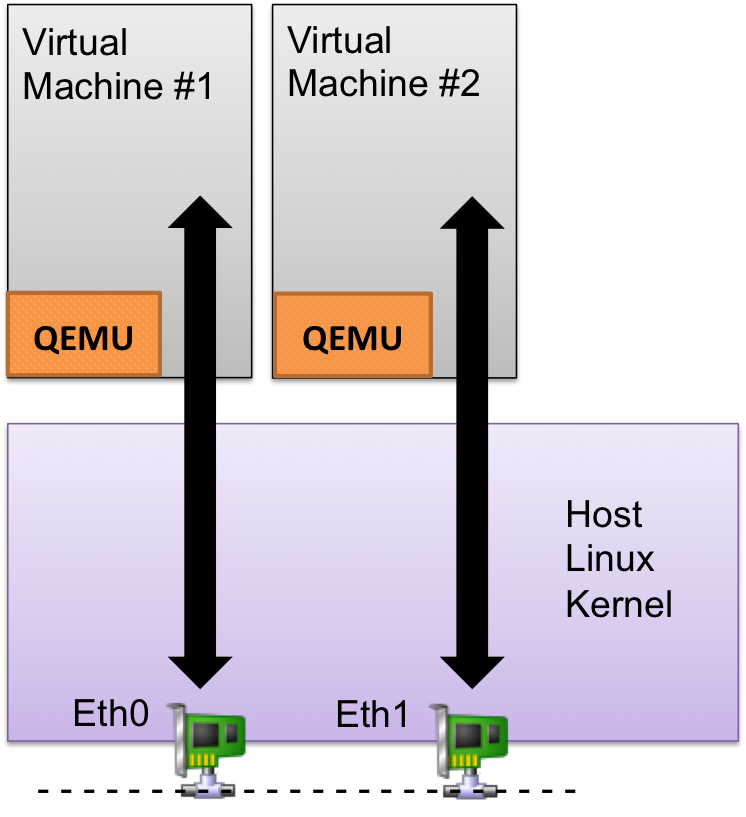
\includegraphics[width=\textwidth]{kvm-direct.png}
                \caption{Direct Device Assignment}
                \label{fig:kvm-direct}
        \end{subfigure}
\newline \newline
        \begin{subfigure}[b]{0.35\textwidth}
                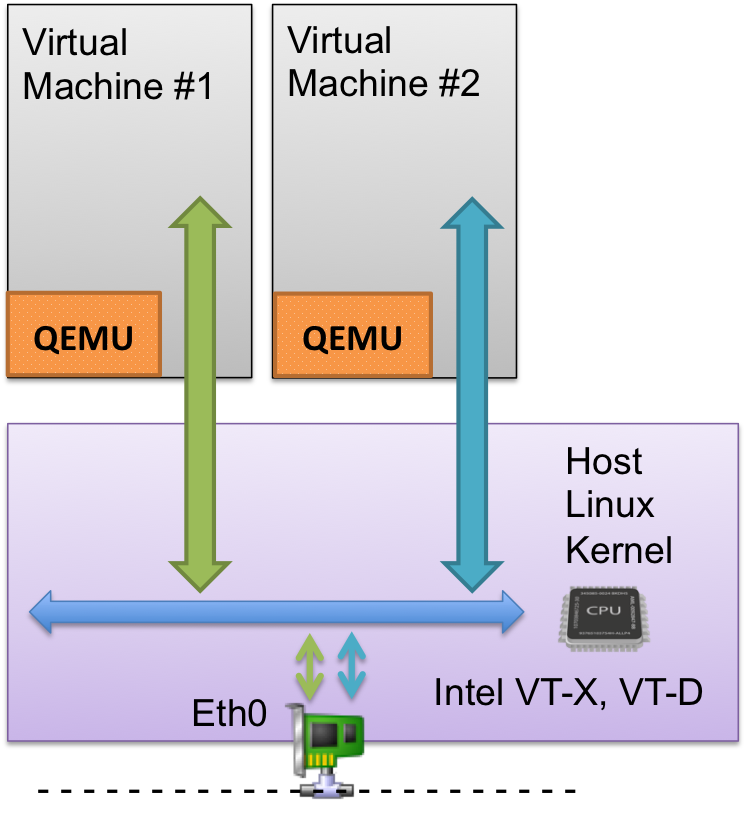
\includegraphics[width=\textwidth]{kvm-direct-sriov.png}
                \caption{Direct Device Assignment with SR-IOV}
                \label{fig:kvm-direct-sriov}
        \end{subfigure}
        \caption{Common Networking options for KVM}\label{fig:kvm-networking}
\end{figure}


Figure \ref{fig:kvm-networking} shows the most common virtual networking options in a KVM based infrastructure.



Figure \ref{fig:kvm-emulated} shows a virtual networking configuration where unmodified guest operating systems can use their native drivers to interact with their virtual network devices. These virtual network devices from the virtual machines are connected to the Tap devices \cite{Tap_devices} on the host kernel. Tap interfaces are software-only interfaces that live only in the kernel and they relay the ethernet frames to and from the linux bridge.This setup trades performance to achieve superior compatibility.



Figure \ref{fig:kvm-para} shows a type of networking where the guest operating system running in the virtual machine is "virtualization aware" and co-operates with the host bypassing the device emulation by QEMU and is known as para-virtualized networking. Para-virtualized networking trades the compatibility to achieve near-native performance.



Figure \ref{fig:kvm-internal} shows a combination of both public and private networking to bring out two facts, first, a virtual machine may have multiple virtual devices second, virtual machines can be privately networked using a linux bridge that is not backed by a physical ethernet device. This setup greatly increases the inter-virtual machine communication performance as the packets need not leave the server to a real networking hardware. This is an ideal networking configuration for a publicly accessible virtual machine to communicate with the secure private virtual machines.Example, a publicly accessible Application server communicating with privately networked database server.



To support the virtualization of network intensive applications, physical network interfaces attached to the host can be directly assigned to the virtual machine bypassing the host kernel and QEMU as shown in Figure \ref{fig:kvm-direct}. This setup provides bare-metal performance due to the direct access to the hardware and is applicable when individual hardware devices are available to be dedicated to the virtual machines. The key to achieve this direct device access is the hardware assistance provided in the form of Intel VT-D \cite{intelvtd}, AMD-IOMMU \cite{amd-iommu}.Intel VT-D and AMD-IOMMU enable secure PCI-pass through to allow the guest operating system in the virtual machine to control the hardware on the host.



Figure \ref{fig:kvm-direct-sriov} shows a networking setup that utilizes ethernet hardware capable of Intel Single Root Input/Output Virtualization (SR-IOV) \cite{sr-iov_primer}. SR-IOV feature takes a step further than the direct device assignment by letting a single hardware be accessed directly by multiple virtual machines with their own configuration space and interrupts. This enables a capable network card to appear as several virtual devices to be directly accessed by the virtual machines.


\textbf{Advanced Networking for the Virtual Machines : }  Virtual LAN (VLAN) provide the capability to create logically separate networks that share the same physical medium. In a virtualized environment, VLANs created for the virtual machines may share the physical network interfaces or share the bridged interface.


\end{enumerate}


%A good technical discussion on how KVM works ... Refer the papers that already did this .... Add more info. Google it.
%Add a nice block diagram of KVM..
%\begin{figure}[htbp]
%\centering
%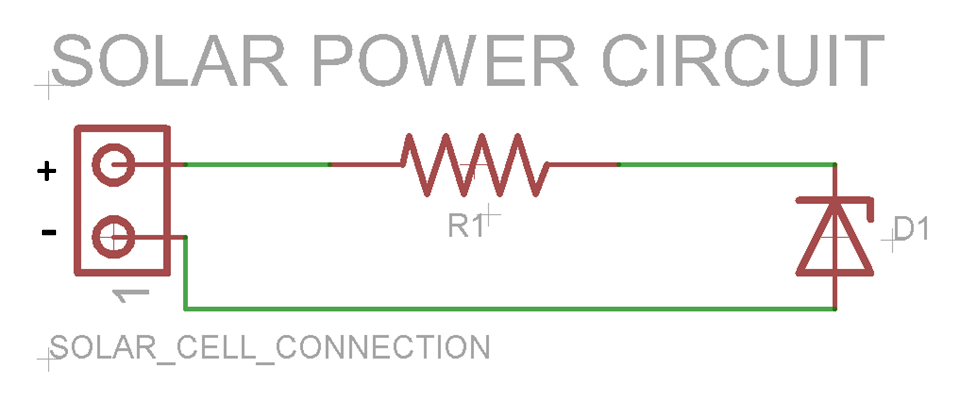
\includegraphics[width=110mm]{solar_pwr_ckt.PNG}
%\caption{Solar Power Circuit}
%\label{img_solarPowerCircuit}
%\end{figure}
%
%As shown in Figure \ref{img_solarPowerCircuit}, Explain the block diagram in detail ..... As shown in Figure \ref{img_solarPowerCircuit}, 
%
%
%Add more detailed tech discussions ... See anatomy of KVM, Developerworks article by Tim Jones ... 
%
%\begin{tabular}{lllp{10cm}}
%where, & • & • & • \\ 
%• & $R$ & = & Resistance ($ohms$) \\ 
%• & $V_{s}$ & = & Output voltage of solar cell ($volts$) \\ 
%• & $V_{z}$ & = & Breakdown voltage of zener diode ($volts$) \\ 
%• & $I_{r}$ & = & Amount of current required by circuit ($mA$) \\ 
% &  &  &  \\ 
%\end{tabular} 
%

\section{Linux Containers}

%Linux Containers are a lightweight operating system virtualization technology. virtualization with Containers is the newest entrant into the linux virtualization arena. There is also an interesting perspective from the Linux community that hypervisors originated due to the linux kernel's incompetence to provide superior resource isolation and effective scale \cite{linux_incompetent} and Containers are the way for the linux kernel to fix them. The core idea is to isolate only a set of processes and their resources in \emph{"Containers"} without involving any device emulation or creating any dependency on the host hardware. Like virtual machines, several containers can run simultaneously on a single host, but all of them share the host kernel for their operation. Isolated containers run directly on the bare-metal hardware using the device drivers native to the host kernel without any intermediate relays. 


%The idea of containers is not new. Solaris Zones [cite], BSD Jails [cite], and Chroot have been around for a long time and are considered as the predecessors for Linux Containers. BSD Jails were designed with an objective of restricting the visibility of the host's resources to a process. For example, when a process runs inside a jail, its root directory is changed to a sub-directory on the host thereby limiting the extent of the file system the process can access. Each process in a jail is provided its own directory sub tree, an IP address defined as an alias to the interface on the host, and optionally a hostname that resolves to its own IP address.

%Linux Containers expanded the scope of BSD jails, and provides a granular operating system virtualization platform to the extent where, containers can be isolated from each other running their own operating system yet sharing the kernel with the host. Containers are provided their own independent file system and network stack. Every container can run its own linux distribution of linux that is different from the host. For example, a host server running RedHat Enterprise Linux [cite] may run containers that run Debian [cite], Ubuntu [cite], CentOS [cite] etc. or even another copy of RedHat Enterprise Linux. This level of abstraction in the containers create an illusion of running virtual machines as discussed earlier with KVM.  

%\begin{figure}[htbp]
%\centering
%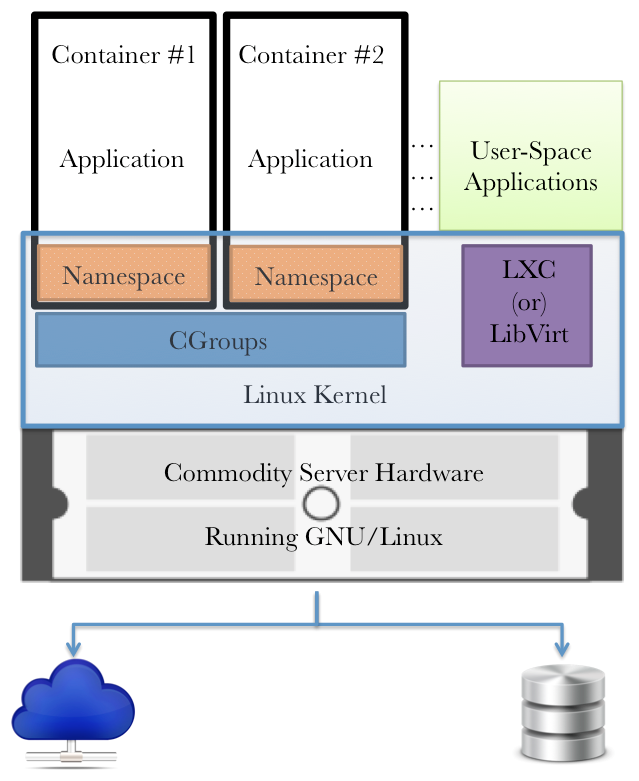
\includegraphics[width=130mm]{lxc-arch.png}
%\caption{Linux Containers - Architecture}
%\label{img_lxc_arch}
%\end{figure}

%Figure \ref{img_lxc_arch} shows the architecture of a server that uses linux containers for virtualization. Unlike KVM, linux containers does not require any assistance from the hardware therefore runs on any hardware that is capable of running the mainline linux kernel. The linux kernel facilitates the execution of containers by the implementation of namespaces at various levels. write about lxc architecture, namespaces, cgroups and that user space applications can co-exist.




Linux Containers are a lightweight operating system virtualization technology. virtualization with Containers is the newest entrant into the linux virtualization arena. There is an interesting perspective from the Linux community that hypervisors originated due to the linux kernel's incompetence to provide superior resource isolation and effective scale \cite{linux_incompetent} and Containers are the way for the linux kernel to fix them. Digging deeper, Hypervisors were created to thoroughly isolate the workloads and to create virtual operating environments, with individual kernels optimally configured in accordance to the workload requirements. But, the key question to be answered is,


\emph{Isn't it the responsibility of an operating system to flexibly isolate its own workloads ?}



If the linux kernel can stand up to solve this problem without the overhead and complexity of running several individual kernels, there would not be a need for hypervisors!


The linux community saw a partial solution to the problem in BSD Jails \cite{jails}, Solaris Zones \cite{zones}, Chroot \cite{chroot}, and most importantly OpenVZ \cite{openvz} - a fork of the linux kernel by Parallels. BSD Jails were designed with an objective of restricting the visibility of the host's resources to a process. For example, when a process runs inside a jail, its root directory is changed to a sub-directory on the host thereby limiting the extent of the file system the process can access. Each process in a jail is provided its own directory sub tree, an IP address defined as an alias to the interface on the host, and optionally a hostname that resolves to the jail's own IP address. The linux kernel's approach to solve the problem was \emph{"Containers"} incorporating the niceties from all the mentioned inspirations and more. 


The core idea is to isolate only a set of processes and their resources in \emph{"Containers"} without involving any device emulation or creating any dependency on the host hardware. Like virtual machines, several containers can run simultaneously on a single host, but all of them share the host kernel for their operation. Isolated containers run directly on the bare-metal hardware using the device drivers native to the host kernel without any intermediate relays. 


Linux Containers expanded the scope of BSD jails, and provides a granular operating system virtualization platform to the extent where, containers can be isolated from each other running their own operating system yet sharing the kernel with the host. Containers are provided their own independent file system and network stack. Every container can run its own linux distribution of linux that is different from the host. For example, a host server running RedHat Enterprise Linux \cite{rhel} may run containers that run Debian \cite{debian}, Ubuntu \cite{ubuntu}, CentOS \cite{centos} etc. or even another copy of RedHat Enterprise Linux. This level of abstraction in the containers create an illusion of running virtual machines as discussed earlier with KVM.  

\begin{figure}[htbp]
\centering
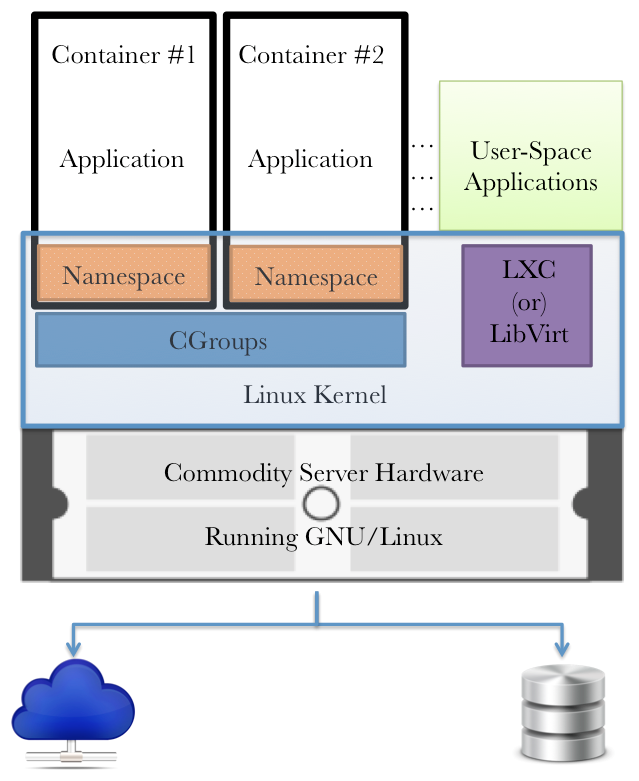
\includegraphics[width=130mm]{lxc-arch.png}
\caption{Linux Containers - Architecture}
\label{img_lxc_arch}
\end{figure}

Figure \ref{img_lxc_arch} shows the architecture of a server that uses linux containers for virtualization. Unlike KVM, linux containers does not require any assistance from the hardware therefore runs on any hardware that is capable of running the mainline linux kernel. The linux kernel facilitates the execution of containers by the implementation of \emph{namespaces} and \emph{cgroups}. 


The following description of namespaces in the linux kernel is based on [cite], [cite], [cite], [cite] by Michael Kerrisk.

%A synopsis of the implementation of namespaces in the linux kernel described by Michael Kerrisk in [cite], [cite], [cite], [cite] :-
%The inclusion of namespaces into the linux kernel was described in detail by Michael Kerrisk through a series of articles. The following discussion on various namespaces at various levels. write about lxc architecture, namespaces, cgroups and that user space applications can co-exist.


Namespaces wrap a particular global system resource on the host and makes it appear to the processes within the namespace(containers) that they have their own isolated instance of the global resource.Linux implements namespaces in 6 categories :- 
\begin{itemize}
\item \textbf{Mount namespaces :}

Mount namespaces enable isolated file system trees to be associated with specific containers(or groups of regular linux processes). A container can create its own file system setup and the subsequent \textit{mount()} and \textit{unmount()} system calls issued by the process would affect only its mount namespace instead of the whole system. For example, multiple containers on the same host can issue \textit{mount()} calls to create a mount point "/data" and access them at "/data" simultaneously. They will reside at a different location on the filesystem tree which will be appropriately seen by the host, say "/\textless containername1\textgreater /data", "/\textless containername2\textgreater /data" and so on. Ofcourse, the same setup can be achieved by using the \textit{chroot()} command. But, chroot can be escaped with certain capabilities including CAP\_SYS\_CHROOT [cite]. Mount namespaces provides a secure alternative. Mount namespaces greatly improves the portability of the containers as they can retain their filesystem trees irrespective of the host's environment.


\item \textbf{UTS namespaces :}

The implementation of UTS namespaces facilitates the containers to issue \textit{sethostname()} and \textit{setdomainname()} system calls to set their own hostname and NIS domain name respectively. \textit{uname()} call issued by the container returns the appropriate hostname and domain name.


\item \textbf{IPC namespaces :}

The implementation of IPC namespaces isolates the System V IPC objects \cite{sysv_ipc} and POSIX Messages queues \cite{posix_msg_queues} associated with individual containers.


\item \textbf{PID namespaces :}

The implementation of PID namespaces in the linux kernel facilitates the isolation of Process IDentification numbers(PID) of the processes running on the host and the processes that are run inside the containers. Every container can have its own init process(PID 1). Several containers running simultaneously can have processes with same PIDs. The linux kernel implements the PIDs as a hierarchy, therefore every process on the host consists of two PIDs (one in the container's namespace and other outside the namespace). This PID abstraction does good in two perspectives, first, isolates the containers such that a process running on one container does not have visibility of processes running on other containers.Second, enables the migration of containers across hosts as the containers can retain the same PIDs.


\item \textbf{Network namespaces :}

The implementation of the network namespaces provides the most useful isolation of network resources for the containers.In other words, it enables the containers to have their own (virtual)network devices, IP addresses, port number space, IP routing tables etc. For example, a single host can run 'n' number of containers each running a web server in its own IP address transparently serving data over port 80.


\item \textbf{User namespaces :}

The implementation of the user namespaces provides the isolation for user and group ID number spaces for the processes running on the directly host and the processes running inside the containers.In other words, a process will have two user and group IDs (one inside the container's namespace and other outside the namespace). This enables an user to posses anUID of 0 (root privileges) inside the container while still being treated as an unprivileged user on the host. The same applies to the application processes that run inside the containers. This abstraction of user privileges greatly improves the security of the container based virtualization solution. It is to be noted that this feature is only available in linux kernel versions 3.8+.
\end{itemize}




Control groups (cgroups) \cite{cgroups} is another key component in the linux kernel that is used for resource management of the containers.

Write about how cgroups manages the resources of containers.
refer its man pages, also browse the blogs

Write about sharing common binaries among the containers for smaller footprint and more performance. 

Write about the relevance of union filesystems (layered operation) and journaled file systems (Easy Snapshotting) and mention CRIU project that allows checkpointing and restart of Linux processes(Containers) that bring live migration to linux containers.

Another innovative perspective upon the idea of containers is coreOS - google more.


%Add a block diagram that shows all the components used in the Linux Containers... cgroups, namespaces, individual filesystems etc..

%\begin{figure}[htbp]
%\centering
%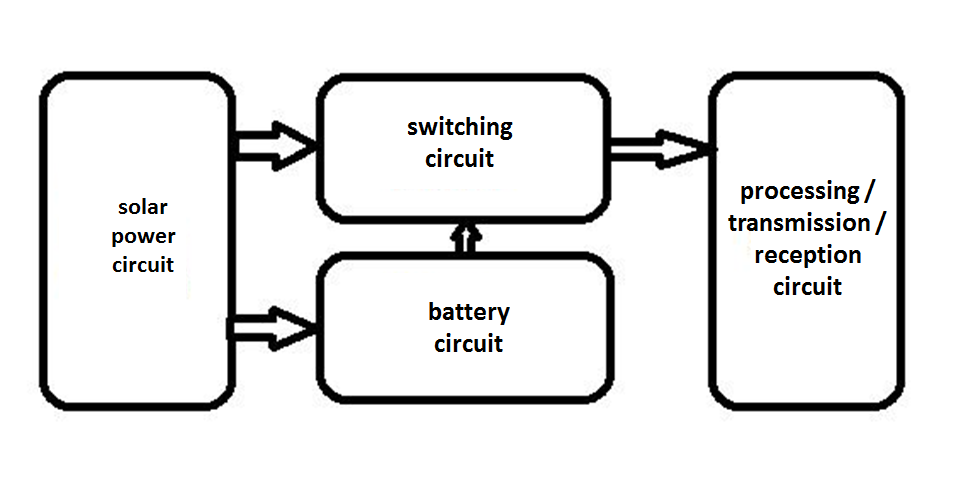
\includegraphics[width=\columnwidth]{block_dia.png}
%\caption{Block Diagram of the Mote Platform}
%\label{img_blockDia}
%\end{figure}
%
%
%Explain the block diagram in detail.
%
%The device works in two modes:
%\begin{enumerate}
%\item Solar Powered:
%The device performs two tasks in solar powered mode. First, it supplies power to the circuit. Second, it charges the Li-Ion battery.
%\item Battery Powered:
%The circuit operates in battery powered mode whenever there is insufficient solar power. The circuit uses power from the Li-Ion battery in this mode.
%\end{enumerate}




\section{Xen}

Same as the above two .. A good technical introduction, followed by a block diagram and more detailed explanation.

%\begin{figure}[htbp]
%\centering
%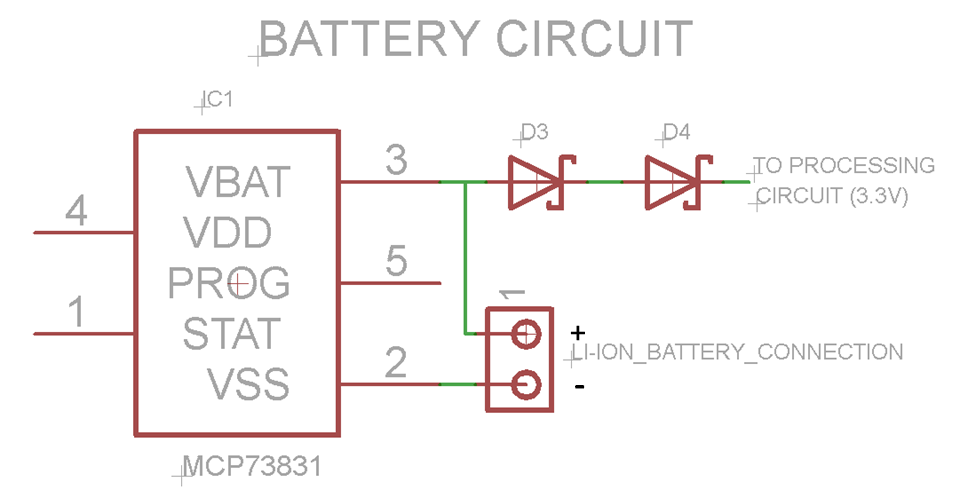
\includegraphics[width=\columnwidth]{battery_ckt.PNG}
%\caption{Battery Circuit}
%\label{img_batteryCircuit}
%\end{figure}
%
%As shown in Figure \ref{img_batteryCircuit}, 